\pgfdeclareplotmark{cross} {
\pgfpathmoveto{\pgfpoint{-0.3\pgfplotmarksize}{\pgfplotmarksize}}
\pgfpathlineto{\pgfpoint{+0.3\pgfplotmarksize}{\pgfplotmarksize}}
\pgfpathlineto{\pgfpoint{+0.3\pgfplotmarksize}{0.3\pgfplotmarksize}}
\pgfpathlineto{\pgfpoint{+1\pgfplotmarksize}{0.3\pgfplotmarksize}}
\pgfpathlineto{\pgfpoint{+1\pgfplotmarksize}{-0.3\pgfplotmarksize}}
\pgfpathlineto{\pgfpoint{+0.3\pgfplotmarksize}{-0.3\pgfplotmarksize}}
\pgfpathlineto{\pgfpoint{+0.3\pgfplotmarksize}{-1.\pgfplotmarksize}}
\pgfpathlineto{\pgfpoint{-0.3\pgfplotmarksize}{-1.\pgfplotmarksize}}
\pgfpathlineto{\pgfpoint{-0.3\pgfplotmarksize}{-0.3\pgfplotmarksize}}
\pgfpathlineto{\pgfpoint{-1.\pgfplotmarksize}{-0.3\pgfplotmarksize}}
\pgfpathlineto{\pgfpoint{-1.\pgfplotmarksize}{0.3\pgfplotmarksize}}
\pgfpathlineto{\pgfpoint{-0.3\pgfplotmarksize}{0.3\pgfplotmarksize}}
\pgfpathclose
\pgfusepathqstroke
}
\pgfdeclareplotmark{cross*} {
\pgfpathmoveto{\pgfpoint{-0.3\pgfplotmarksize}{\pgfplotmarksize}}
\pgfpathlineto{\pgfpoint{+0.3\pgfplotmarksize}{\pgfplotmarksize}}
\pgfpathlineto{\pgfpoint{+0.3\pgfplotmarksize}{0.3\pgfplotmarksize}}
\pgfpathlineto{\pgfpoint{+1\pgfplotmarksize}{0.3\pgfplotmarksize}}
\pgfpathlineto{\pgfpoint{+1\pgfplotmarksize}{-0.3\pgfplotmarksize}}
\pgfpathlineto{\pgfpoint{+0.3\pgfplotmarksize}{-0.3\pgfplotmarksize}}
\pgfpathlineto{\pgfpoint{+0.3\pgfplotmarksize}{-1.\pgfplotmarksize}}
\pgfpathlineto{\pgfpoint{-0.3\pgfplotmarksize}{-1.\pgfplotmarksize}}
\pgfpathlineto{\pgfpoint{-0.3\pgfplotmarksize}{-0.3\pgfplotmarksize}}
\pgfpathlineto{\pgfpoint{-1.\pgfplotmarksize}{-0.3\pgfplotmarksize}}
\pgfpathlineto{\pgfpoint{-1.\pgfplotmarksize}{0.3\pgfplotmarksize}}
\pgfpathlineto{\pgfpoint{-0.3\pgfplotmarksize}{0.3\pgfplotmarksize}}
\pgfpathclose
\pgfusepathqfillstroke
}
\pgfdeclareplotmark{newstar} {
\pgfpathmoveto{\pgfqpoint{0pt}{\pgfplotmarksize}}
\pgfpathlineto{\pgfqpointpolar{44}{0.5\pgfplotmarksize}}
\pgfpathlineto{\pgfqpointpolar{18}{\pgfplotmarksize}}
\pgfpathlineto{\pgfqpointpolar{-20}{0.5\pgfplotmarksize}}
\pgfpathlineto{\pgfqpointpolar{-54}{\pgfplotmarksize}}
\pgfpathlineto{\pgfqpointpolar{-90}{0.5\pgfplotmarksize}}
\pgfpathlineto{\pgfqpointpolar{234}{\pgfplotmarksize}}
\pgfpathlineto{\pgfqpointpolar{198}{0.5\pgfplotmarksize}}
\pgfpathlineto{\pgfqpointpolar{162}{\pgfplotmarksize}}
\pgfpathlineto{\pgfqpointpolar{134}{0.5\pgfplotmarksize}}
\pgfpathclose
\pgfusepathqstroke
}
\pgfdeclareplotmark{newstar*} {
\pgfpathmoveto{\pgfqpoint{0pt}{\pgfplotmarksize}}
\pgfpathlineto{\pgfqpointpolar{44}{0.5\pgfplotmarksize}}
\pgfpathlineto{\pgfqpointpolar{18}{\pgfplotmarksize}}
\pgfpathlineto{\pgfqpointpolar{-20}{0.5\pgfplotmarksize}}
\pgfpathlineto{\pgfqpointpolar{-54}{\pgfplotmarksize}}
\pgfpathlineto{\pgfqpointpolar{-90}{0.5\pgfplotmarksize}}
\pgfpathlineto{\pgfqpointpolar{234}{\pgfplotmarksize}}
\pgfpathlineto{\pgfqpointpolar{198}{0.5\pgfplotmarksize}}
\pgfpathlineto{\pgfqpointpolar{162}{\pgfplotmarksize}}
\pgfpathlineto{\pgfqpointpolar{134}{0.5\pgfplotmarksize}}
\pgfpathclose
\pgfusepathqfillstroke
}
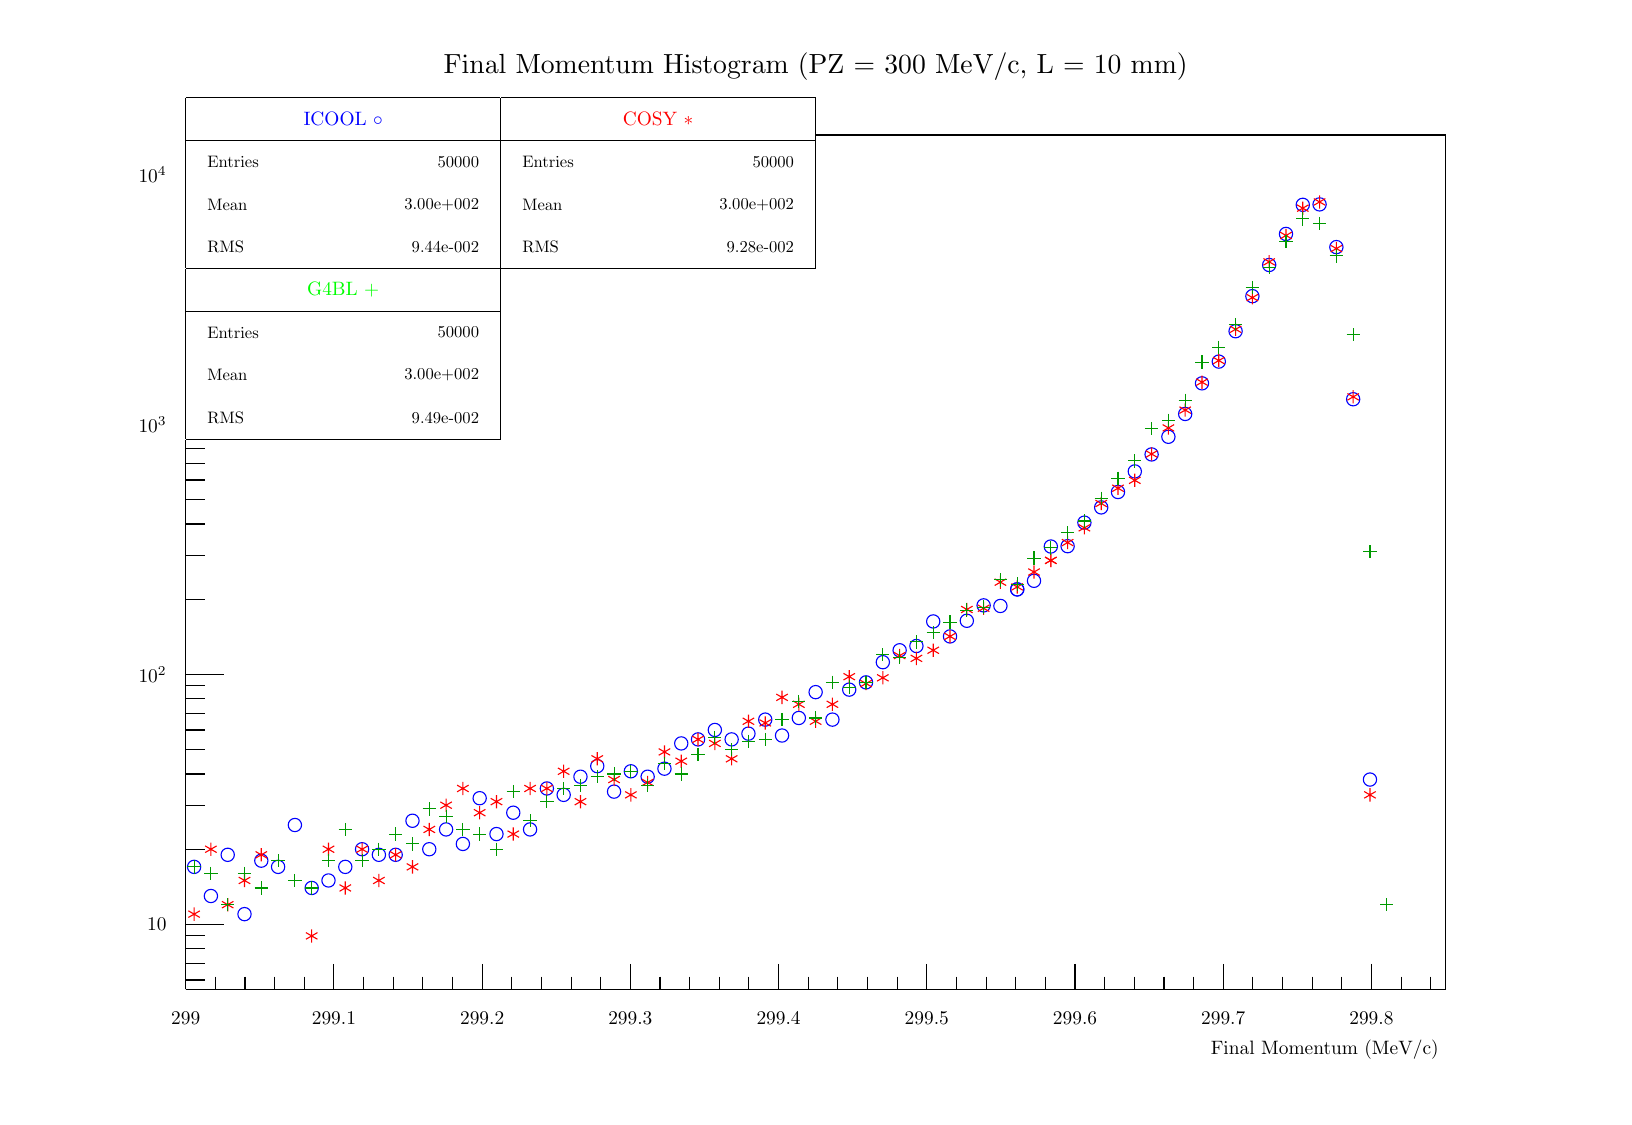
\begin{tikzpicture}
\definecolor{c}{rgb}{1,1,1};
\draw [color=c, fill=c] (0,0) rectangle (20,13.5632);
\draw [color=c, fill=c] (2,1.35632) rectangle (18,12.2069);
\definecolor{c}{rgb}{0,0,0};
\draw [c] (2,1.35632) -- (2,12.2069) -- (18,12.2069) -- (18,1.35632) -- (2,1.35632);
\definecolor{c}{rgb}{1,1,1};
\draw [color=c, fill=c] (2,1.35632) rectangle (18,12.2069);
\definecolor{c}{rgb}{0,0,0};
\draw [c] (2,1.35632) -- (2,12.2069) -- (18,12.2069) -- (18,1.35632) -- (2,1.35632);
\definecolor{c}{rgb}{0,0,1};
\foreach \P in
 {(2.10667,2.9123),(2.32,2.54241),(2.53333,3.06567),(2.74667,2.31207),(2.96,2.99111),(3.17333,2.9123),(3.38667,3.44407),(3.6,2.64459),(3.81333,2.73972),(4.02667,2.9123),(4.24,3.13639),(4.45333,3.06567),(4.66667,3.06567),(4.88,3.49815),(5.09333,3.1363
9),(5.30667,3.38778),(5.52,3.20366),(5.73333,3.78445),(5.94667,3.3291),(6.16,3.60033),(6.37333,3.38778),(6.58667,3.90801),(6.8,3.82688),(7.01333,4.05722),(7.22667,4.19185),(7.44,3.86805),(7.65333,4.12618),(7.86667,4.05722),(8.08,4.15941),(8.29333,4.4
8016),(8.50667,4.53123),(8.72,4.65121),(8.93333,4.53123),(9.14667,4.60446),(9.36,4.78263),(9.57333,4.58048),(9.78667,4.80336),(10,5.13147),(10.2133,4.78263),(10.4267,5.16354),(10.64,5.25549),(10.8533,5.51182),(11.0667,5.66324),(11.28,5.71732),(11.493
3,6.02923),(11.7067,5.83906),(11.92,6.03767),(12.1333,6.2333),(12.3467,6.22599),(12.56,6.43644)}{\draw[mark options={color=c,fill=c},mark size=2.402402pt,mark=o] plot coordinates {\P};}
\foreach \P in
 {(12.56,6.43644),(12.7733,6.54535),(12.9867,6.98074),(13.2,6.98498),(13.4133,7.28417),(13.6267,7.47762),(13.84,7.67316),(14.0533,7.93436),(14.2667,8.15025),(14.48,8.37443),(14.6933,8.66439),(14.9067,9.05322),(15.12,9.3294),(15.3333,9.71502),(15.5467
,10.1603),(15.76,10.5563),(15.9733,10.9505),(16.1867,11.3204),(16.4,11.3257),(16.6133,10.7834),(16.8267,8.85132),(17.04,4.02141)}{\draw[mark options={color=c,fill=c},mark size=2.402402pt,mark=o] plot coordinates {\P};}
\definecolor{c}{rgb}{1,1,1};
\draw [color=c, fill=c] (2,10.5115) rectangle (6,12.6816);
\definecolor{c}{rgb}{0,0,0};
\draw [c] (2,10.5115) -- (6,10.5115);
\draw [c] (6,10.5115) -- (6,12.6816);
\draw [c] (6,12.6816) -- (2,12.6816);
\draw [c] (2,12.6816) -- (2,10.5115);
\draw[color=blue](4,12.4103) node[scale=0.7, rotate=0]{ICOOL $\circ$};
\draw [c] (2,12.1391) -- (6,12.1391);
\draw [anchor= west] (2.2,11.8678) node[scale=0.6, rotate=0]{Entries };
\draw [anchor= east] (5.8,11.8678) node[scale=0.6, rotate=0]{ 50000};
\draw [anchor= west] (2.2,11.3253) node[scale=0.6, rotate=0]{Mean  };
\draw [anchor= east] (5.8,11.3253) node[scale=0.6, rotate=0]{ 3.00e+002};
\draw [anchor= west] (2.2,10.7828) node[scale=0.6, rotate=0]{RMS   };
\draw [anchor= east] (5.8,10.7828) node[scale=0.6, rotate=0]{ 9.44e-002};
\draw [c] (2,1.35632) -- (18,1.35632);
\draw [anchor= east] (18,0.596782) node[scale=0.7, rotate=0]{Final Momentum (MeV/c)};
\draw [c] (2,1.68184) -- (2,1.35632);
\draw [c] (2.37647,1.51908) -- (2.37647,1.35632);
\draw [c] (2.75294,1.51908) -- (2.75294,1.35632);
\draw [c] (3.12941,1.51908) -- (3.12941,1.35632);
\draw [c] (3.50588,1.51908) -- (3.50588,1.35632);
\draw [c] (3.88235,1.68184) -- (3.88235,1.35632);
\draw [c] (4.25882,1.51908) -- (4.25882,1.35632);
\draw [c] (4.63529,1.51908) -- (4.63529,1.35632);
\draw [c] (5.01176,1.51908) -- (5.01176,1.35632);
\draw [c] (5.38824,1.51908) -- (5.38824,1.35632);
\draw [c] (5.76471,1.68184) -- (5.76471,1.35632);
\draw [c] (6.14118,1.51908) -- (6.14118,1.35632);
\draw [c] (6.51765,1.51908) -- (6.51765,1.35632);
\draw [c] (6.89412,1.51908) -- (6.89412,1.35632);
\draw [c] (7.27059,1.51908) -- (7.27059,1.35632);
\draw [c] (7.64706,1.68184) -- (7.64706,1.35632);
\draw [c] (8.02353,1.51908) -- (8.02353,1.35632);
\draw [c] (8.4,1.51908) -- (8.4,1.35632);
\draw [c] (8.77647,1.51908) -- (8.77647,1.35632);
\draw [c] (9.15294,1.51908) -- (9.15294,1.35632);
\draw [c] (9.52941,1.68184) -- (9.52941,1.35632);
\draw [c] (9.90588,1.51908) -- (9.90588,1.35632);
\draw [c] (10.2824,1.51908) -- (10.2824,1.35632);
\draw [c] (10.6588,1.51908) -- (10.6588,1.35632);
\draw [c] (11.0353,1.51908) -- (11.0353,1.35632);
\draw [c] (11.4118,1.68184) -- (11.4118,1.35632);
\draw [c] (11.7882,1.51908) -- (11.7882,1.35632);
\draw [c] (12.1647,1.51908) -- (12.1647,1.35632);
\draw [c] (12.5412,1.51908) -- (12.5412,1.35632);
\draw [c] (12.9176,1.51908) -- (12.9176,1.35632);
\draw [c] (13.2941,1.68184) -- (13.2941,1.35632);
\draw [c] (13.6706,1.51908) -- (13.6706,1.35632);
\draw [c] (14.0471,1.51908) -- (14.0471,1.35632);
\draw [c] (14.4235,1.51908) -- (14.4235,1.35632);
\draw [c] (14.8,1.51908) -- (14.8,1.35632);
\draw [c] (15.1765,1.68184) -- (15.1765,1.35632);
\draw [c] (15.5529,1.51908) -- (15.5529,1.35632);
\draw [c] (15.9294,1.51908) -- (15.9294,1.35632);
\draw [c] (16.3059,1.51908) -- (16.3059,1.35632);
\draw [c] (16.6824,1.51908) -- (16.6824,1.35632);
\draw [c] (17.0588,1.68184) -- (17.0588,1.35632);
\draw [c] (17.0588,1.68184) -- (17.0588,1.35632);
\draw [c] (17.4353,1.51908) -- (17.4353,1.35632);
\draw [c] (17.8118,1.51908) -- (17.8118,1.35632);
\draw [anchor=base] (2,0.908736) node[scale=0.7, rotate=0]{299};
\draw [anchor=base] (3.88235,0.908736) node[scale=0.7, rotate=0]{299.1};
\draw [anchor=base] (5.76471,0.908736) node[scale=0.7, rotate=0]{299.2};
\draw [anchor=base] (7.64706,0.908736) node[scale=0.7, rotate=0]{299.3};
\draw [anchor=base] (9.52941,0.908736) node[scale=0.7, rotate=0]{299.4};
\draw [anchor=base] (11.4118,0.908736) node[scale=0.7, rotate=0]{299.5};
\draw [anchor=base] (13.2941,0.908736) node[scale=0.7, rotate=0]{299.6};
\draw [anchor=base] (15.1765,0.908736) node[scale=0.7, rotate=0]{299.7};
\draw [anchor=base] (17.0588,0.908736) node[scale=0.7, rotate=0]{299.8};
\draw [c] (2,1.35632) -- (2,12.2069);
\draw [c] (2.24,1.47629) -- (2,1.47629);
\draw [c] (2.24,1.68884) -- (2,1.68884);
\draw [c] (2.24,1.87296) -- (2,1.87296);
\draw [c] (2.24,2.03537) -- (2,2.03537);
\draw [c] (2.48,2.18064) -- (2,2.18064);
\draw [anchor= east] (1.844,2.18064) node[scale=0.7, rotate=0]{10};
\draw [c] (2.24,3.13639) -- (2,3.13639);
\draw [c] (2.24,3.69546) -- (2,3.69546);
\draw [c] (2.24,4.09213) -- (2,4.09213);
\draw [c] (2.24,4.39981) -- (2,4.39981);
\draw [c] (2.24,4.65121) -- (2,4.65121);
\draw [c] (2.24,4.86376) -- (2,4.86376);
\draw [c] (2.24,5.04788) -- (2,5.04788);
\draw [c] (2.24,5.21028) -- (2,5.21028);
\draw [c] (2.48,5.35556) -- (2,5.35556);
\draw [anchor= east] (1.844,5.35556) node[scale=0.7, rotate=0]{$10^{2}$};
\draw [c] (2.24,6.3113) -- (2,6.3113);
\draw [c] (2.24,6.87037) -- (2,6.87037);
\draw [c] (2.24,7.26704) -- (2,7.26704);
\draw [c] (2.24,7.57472) -- (2,7.57472);
\draw [c] (2.24,7.82612) -- (2,7.82612);
\draw [c] (2.24,8.03867) -- (2,8.03867);
\draw [c] (2.24,8.22279) -- (2,8.22279);
\draw [c] (2.24,8.38519) -- (2,8.38519);
\draw [c] (2.48,8.53047) -- (2,8.53047);
\draw [anchor= east] (1.844,8.53047) node[scale=0.7, rotate=0]{$10^{3}$};
\draw [c] (2.24,9.48621) -- (2,9.48621);
\draw [c] (2.24,10.0453) -- (2,10.0453);
\draw [c] (2.24,10.442) -- (2,10.442);
\draw [c] (2.24,10.7496) -- (2,10.7496);
\draw [c] (2.24,11.001) -- (2,11.001);
\draw [c] (2.24,11.2136) -- (2,11.2136);
\draw [c] (2.24,11.3977) -- (2,11.3977);
\draw [c] (2.24,11.5601) -- (2,11.5601);
\draw [c] (2.48,11.7054) -- (2,11.7054);
\draw [anchor= east] (1.844,11.7054) node[scale=0.7, rotate=0]{$10^{4}$};
\definecolor{c}{rgb}{1,1,1};
\draw [color=c, fill=c] (2,10.5115) rectangle (6,12.6816);
\definecolor{c}{rgb}{0,0,0};
\draw [c] (2,10.5115) -- (6,10.5115);
\draw [c] (6,10.5115) -- (6,12.6816);
\draw [c] (6,12.6816) -- (2,12.6816);
\draw [c] (2,12.6816) -- (2,10.5115);
\draw[color=blue](4,12.4103) node[scale=0.7, rotate=0]{ICOOL $\circ$};
\draw [c] (2,12.1391) -- (6,12.1391);
\draw [anchor= west] (2.2,11.8678) node[scale=0.6, rotate=0]{Entries };
\draw [anchor= east] (5.8,11.8678) node[scale=0.6, rotate=0]{ 50000};
\draw [anchor= west] (2.2,11.3253) node[scale=0.6, rotate=0]{Mean  };
\draw [anchor= east] (5.8,11.3253) node[scale=0.6, rotate=0]{ 3.00e+002};
\draw [anchor= west] (2.2,10.7828) node[scale=0.6, rotate=0]{RMS   };
\draw [anchor= east] (5.8,10.7828) node[scale=0.6, rotate=0]{ 9.44e-002};
\draw (10,13.0816) node[scale=1, rotate=0]{Final Momentum Histogram (PZ = 300 MeV/c, L = 10 mm)};
\definecolor{c}{rgb}{1,0,0};
\foreach \P in
 {(2.10667,2.31207),(2.32,3.13639),(2.53333,2.43204),(2.74667,2.73972),(2.96,3.06567),(3.6,2.03537),(3.81333,3.13639),(4.02667,2.64459),(4.24,3.13639),(4.45333,2.73972),(4.66667,3.06567),(4.88,2.9123),(5.09333,3.38778),(5.30667,3.69546),(5.52,3.90801
),(5.73333,3.60033),(5.94667,3.74068),(6.16,3.3291),(6.37333,3.90801),(6.58667,3.90801),(6.8,4.12618),(7.01333,3.74068),(7.22667,4.28484),(7.44,4.02141),(7.65333,3.82688),(7.86667,3.98464),(8.08,4.37196),(8.29333,4.25454),(8.50667,4.53123),(8.72,4.48
016),(8.93333,4.28484),(9.14667,4.76157),(9.36,4.7402),(9.57333,5.06501),(9.78667,4.97715),(10,4.76157),(10.2133,4.97715),(10.4267,5.3277),(10.64,5.24059),(10.8533,5.31356),(11.0667,5.59541),(11.28,5.56021),(11.4933,5.66324),(11.7067,5.83906),(11.92,
6.18126),(12.1333,6.19633),(12.3467,6.52779),(12.56,6.46756),(12.7733,6.65706),(12.9867,6.80448)}{\draw[mark options={color=c,fill=c},mark size=2.402402pt,mark=asterisk] plot coordinates {\P};}
\foreach \P in
 {(12.9867,6.80448),(13.2,7.03074),(13.4133,7.21792),(13.6267,7.52703),(13.84,7.7211),(14.0533,7.82152),(14.2667,8.15569),(14.48,8.48705),(14.6933,8.71355),(14.9067,9.06824),(15.12,9.34247),(15.3333,9.73933),(15.5467,10.142),(15.76,10.5961),(15.9733,
10.9308),(16.1867,11.2777),(16.4,11.3569),(16.6133,10.7644),(16.8267,8.88158),(17.04,3.82688)}{\draw[mark options={color=c,fill=c},mark size=2.402402pt,mark=asterisk] plot coordinates {\P};}
\definecolor{c}{rgb}{1,1,1};
\draw [color=c, fill=c] (6,10.5115) rectangle (10,12.6816);
\definecolor{c}{rgb}{0,0,0};
\draw [c] (6,10.5115) -- (10,10.5115);
\draw [c] (10,10.5115) -- (10,12.6816);
\draw [c] (10,12.6816) -- (6,12.6816);
\draw [c] (6,12.6816) -- (6,10.5115);
\draw [color=red](8,12.4103) node[scale=0.7, rotate=0]{COSY $*$};
\draw [c] (6,12.1391) -- (10,12.1391);
\draw [anchor= west] (6.2,11.8678) node[scale=0.6, rotate=0]{Entries };
\draw [anchor= east] (9.8,11.8678) node[scale=0.6, rotate=0]{ 50000};
\draw [anchor= west] (6.2,11.3253) node[scale=0.6, rotate=0]{Mean  };
\draw [anchor= east] (9.8,11.3253) node[scale=0.6, rotate=0]{ 3.00e+002};
\draw [anchor= west] (6.2,10.7828) node[scale=0.6, rotate=0]{RMS   };
\draw [anchor= east] (9.8,10.7828) node[scale=0.6, rotate=0]{ 9.28e-002};
\definecolor{c}{rgb}{1,1,1};
\draw [color=c, fill=c] (6,10.5115) rectangle (10,12.6816);
\definecolor{c}{rgb}{0,0,0};
\draw [c] (6,10.5115) -- (10,10.5115);
\draw [c] (10,10.5115) -- (10,12.6816);
\draw [c] (10,12.6816) -- (6,12.6816);
\draw [c] (6,12.6816) -- (6,10.5115);
\draw [color=red](8,12.4103) node[scale=0.7, rotate=0]{COSY $*$};
\draw [c] (6,12.1391) -- (10,12.1391);
\draw [anchor= west] (6.2,11.8678) node[scale=0.6, rotate=0]{Entries };
\draw [anchor= east] (9.8,11.8678) node[scale=0.6, rotate=0]{ 50000};
\draw [anchor= west] (6.2,11.3253) node[scale=0.6, rotate=0]{Mean  };
\draw [anchor= east] (9.8,11.3253) node[scale=0.6, rotate=0]{ 3.00e+002};
\draw [anchor= west] (6.2,10.7828) node[scale=0.6, rotate=0]{RMS   };
\draw [anchor= east] (9.8,10.7828) node[scale=0.6, rotate=0]{ 9.28e-002};
\definecolor{c}{rgb}{0,0.6,0};
\foreach \P in
 {(2.10667,2.9123),(2.32,2.82871),(2.53333,2.43204),(2.74667,2.82871),(2.96,2.64459),(3.17333,2.99111),(3.38667,2.73972),(3.6,2.64459),(3.81333,2.99111),(4.02667,3.38778),(4.24,2.99111),(4.45333,3.13639),(4.66667,3.3291),(4.88,3.20366),(5.09333,3.648
72),(5.30667,3.55019),(5.52,3.38778),(5.73333,3.3291),(5.94667,3.13639),(6.16,3.86805),(6.37333,3.49815),(6.58667,3.74068),(6.8,3.90801),(7.01333,3.94686),(7.22667,4.05722),(7.44,4.09213),(7.65333,4.12618),(7.86667,3.94686),(8.08,4.22355),(8.29333,4.
09213),(8.50667,4.34353),(8.72,4.55608),(8.93333,4.39981),(9.14667,4.50593),(9.36,4.53123),(9.57333,4.78263),(9.78667,5.01297),(10,4.80336),(10.2133,5.25549),(10.4267,5.19488),(10.64,5.25549),(10.8533,5.60695),(11.0667,5.57204),(11.28,5.76936),(11.49
33,5.88678),(11.7067,6.02075),(11.92,6.17366),(12.1333,6.21124),(12.3467,6.55694),(12.56,6.50401)}{\draw[mark options={color=c,fill=c},mark size=2.402402pt,mark=+] plot coordinates {\P};}
\foreach \P in
 {(12.56,6.50401),(12.7733,6.83311),(12.9867,6.96367),(13.2,7.15582),(13.4133,7.30445),(13.6267,7.5939),(13.84,7.84891),(14.0533,8.0679),(14.2667,8.47562),(14.48,8.58455),(14.6933,8.83705),(14.9067,9.32243),(15.12,9.51081),(15.3333,9.80159),(15.5467,
10.2708),(15.76,10.5268),(15.9733,10.8514),(16.1867,11.1414),(16.4,11.0812),(16.6133,10.6711),(16.8267,9.6699),(17.04,6.91559),(17.2533,2.43204)}{\draw[mark options={color=c,fill=c},mark size=2.402402pt,mark=+] plot coordinates {\P};}
\definecolor{c}{rgb}{1,1,1};
\draw [color=c, fill=c] (2,8.34138) rectangle (6,10.5115);
\definecolor{c}{rgb}{0,0,0};
\draw [c] (2,8.34138) -- (6,8.34138);
\draw [c] (6,8.34138) -- (6,10.5115);
\draw [c] (6,10.5115) -- (2,10.5115);
\draw [c] (2,10.5115) -- (2,8.34138);
\draw [color=green](4,10.2402) node[scale=0.7, rotate=0]{G4BL $+$};
\draw [c] (2,9.96897) -- (6,9.96897);
\draw [anchor= west] (2.2,9.6977) node[scale=0.6, rotate=0]{Entries };
\draw [anchor= east] (5.8,9.6977) node[scale=0.6, rotate=0]{ 50000};
\draw [anchor= west] (2.2,9.15517) node[scale=0.6, rotate=0]{Mean  };
\draw [anchor= east] (5.8,9.15517) node[scale=0.6, rotate=0]{ 3.00e+002};
\draw [anchor= west] (2.2,8.61264) node[scale=0.6, rotate=0]{RMS   };
\draw [anchor= east] (5.8,8.61264) node[scale=0.6, rotate=0]{ 9.49e-002};
\definecolor{c}{rgb}{1,1,1};
\draw [color=c, fill=c] (2,8.34138) rectangle (6,10.5115);
\definecolor{c}{rgb}{0,0,0};
\draw [c] (2,8.34138) -- (6,8.34138);
\draw [c] (6,8.34138) -- (6,10.5115);
\draw [c] (6,10.5115) -- (2,10.5115);
\draw [c] (2,10.5115) -- (2,8.34138);
\draw [color=green](4,10.2402) node[scale=0.7, rotate=0]{G4BL $+$};
\draw [c] (2,9.96897) -- (6,9.96897);
\draw [anchor= west] (2.2,9.6977) node[scale=0.6, rotate=0]{Entries };
\draw [anchor= east] (5.8,9.6977) node[scale=0.6, rotate=0]{ 50000};
\draw [anchor= west] (2.2,9.15517) node[scale=0.6, rotate=0]{Mean  };
\draw [anchor= east] (5.8,9.15517) node[scale=0.6, rotate=0]{ 3.00e+002};
\draw [anchor= west] (2.2,8.61264) node[scale=0.6, rotate=0]{RMS   };
\draw [anchor= east] (5.8,8.61264) node[scale=0.6, rotate=0]{ 9.49e-002};
\end{tikzpicture}
